\documentclass[tikz,border=7pt]{standalone}
\usepackage{amsmath,amssymb}
\usetikzlibrary{arrows.meta,positioning,calc,shapes.geometric}

\begin{document}
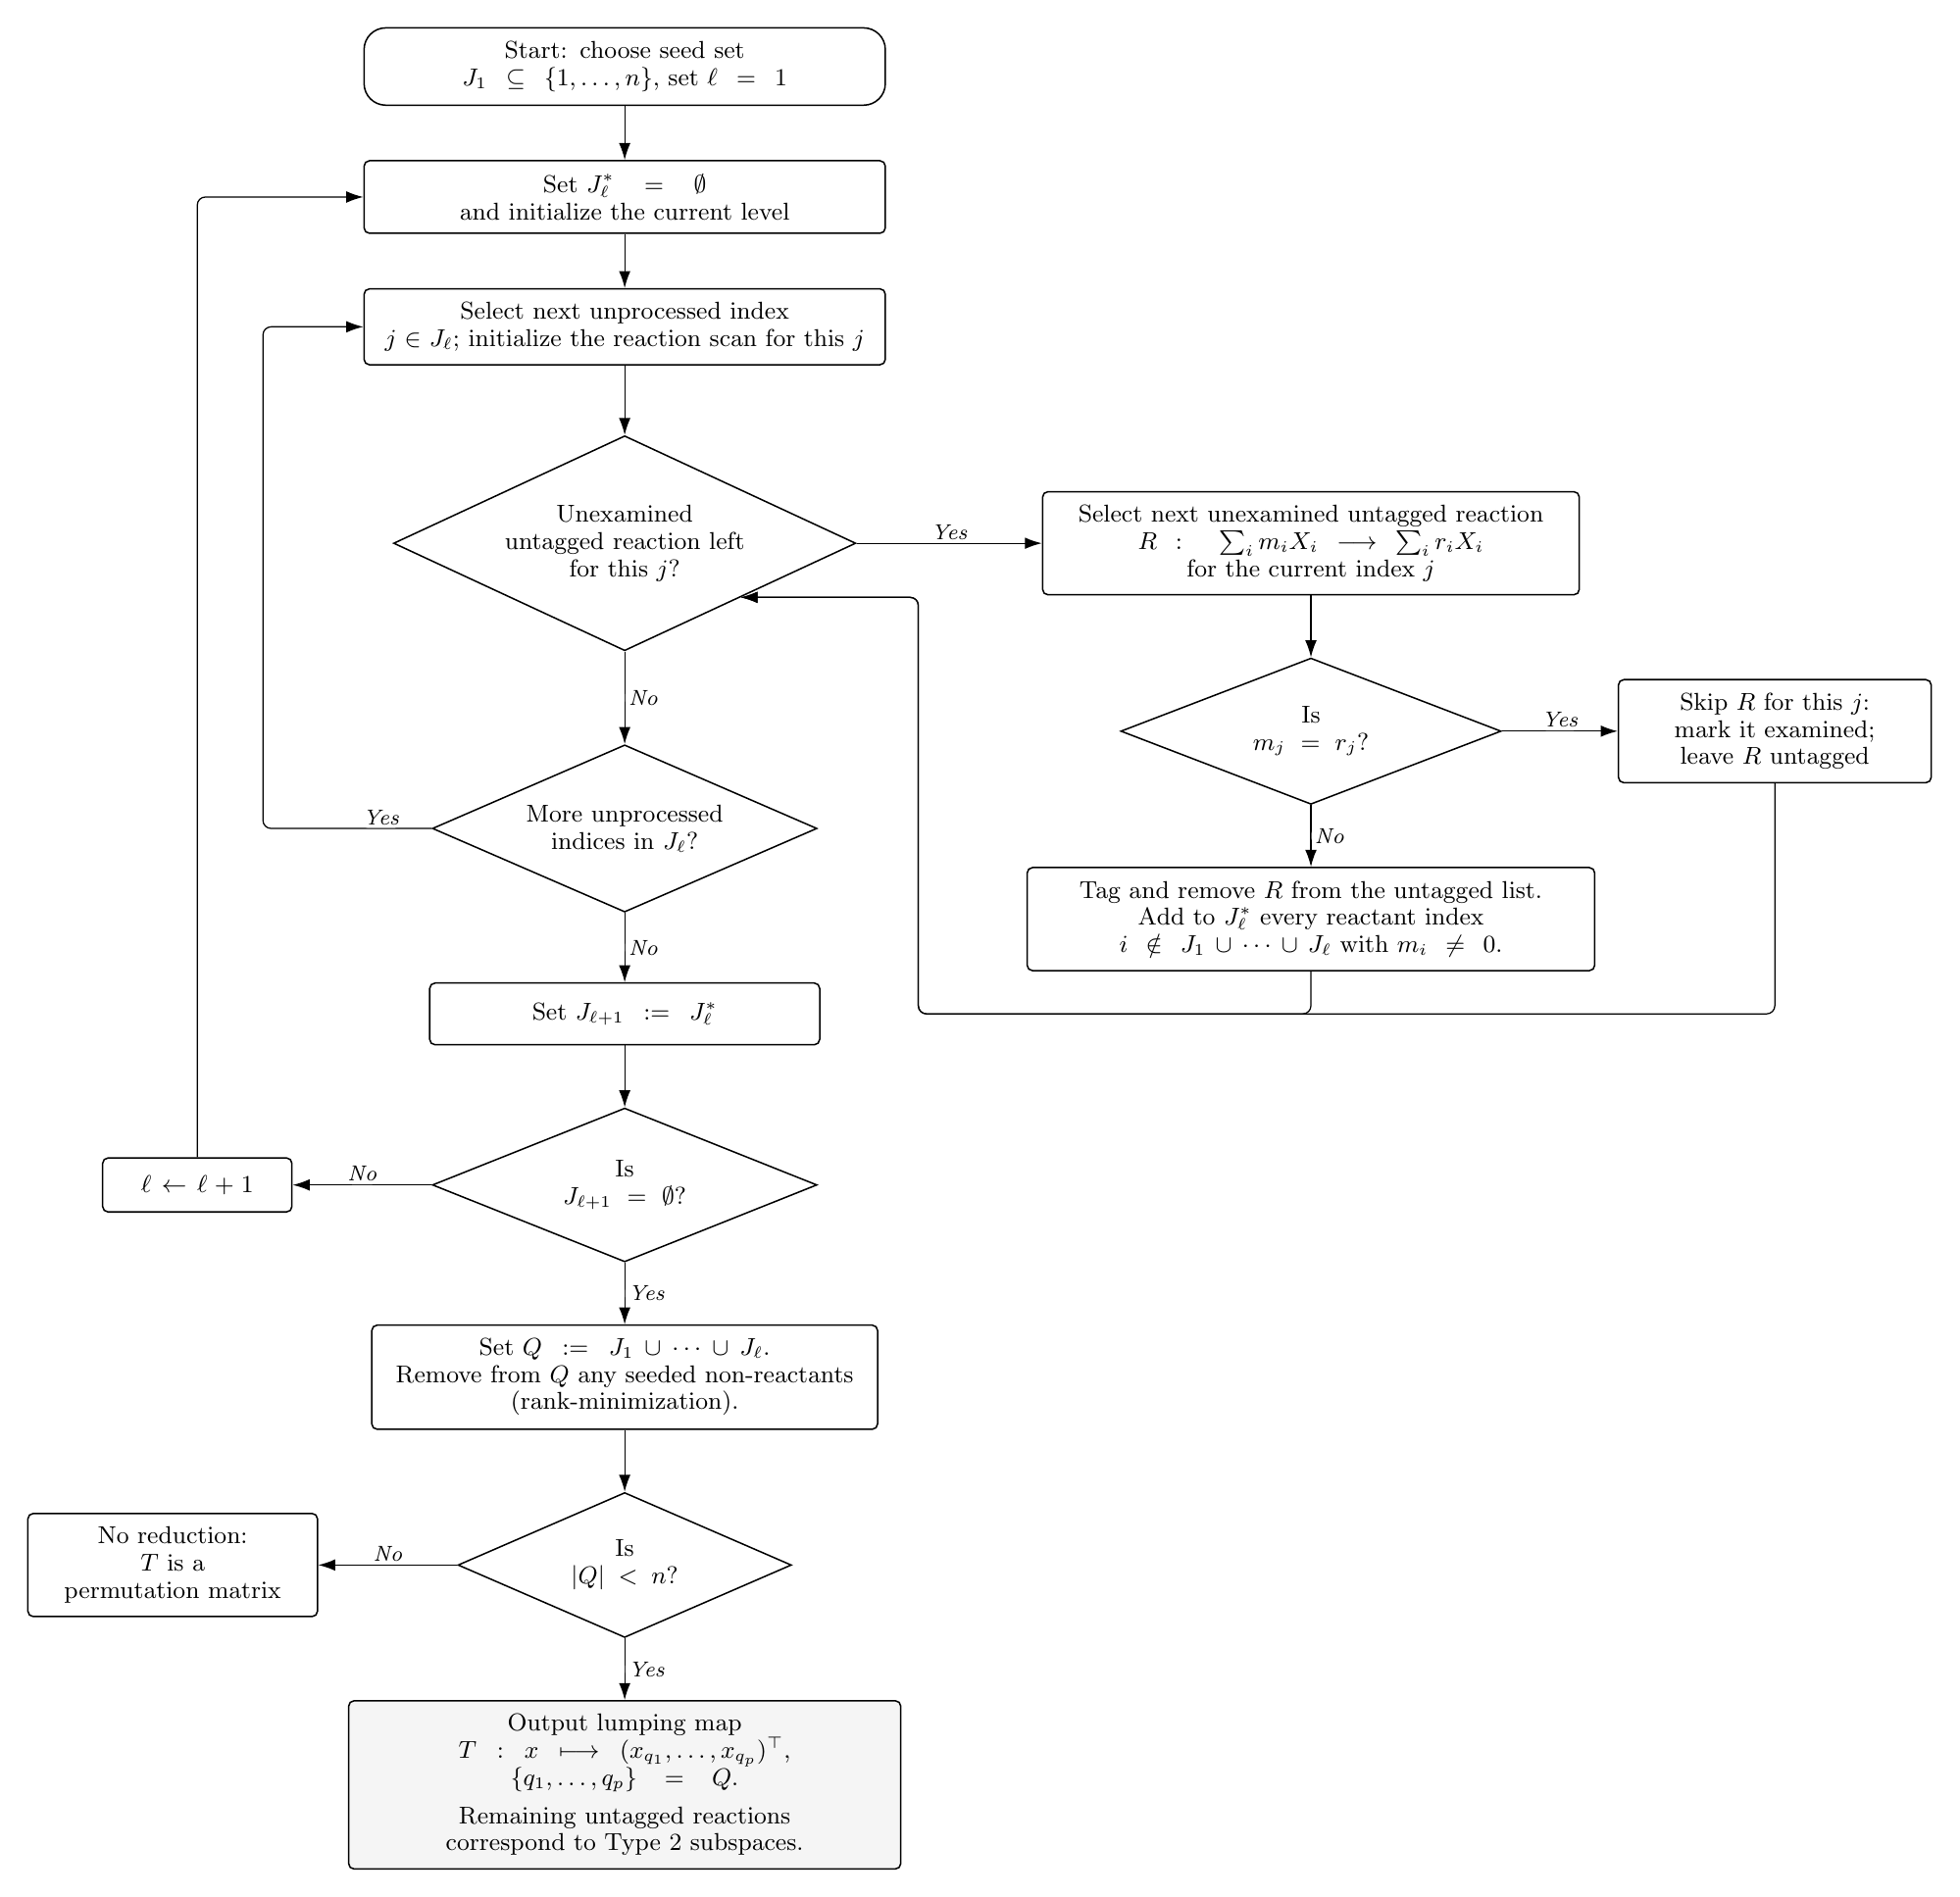
\begin{tikzpicture}[
  >=Latex,
  line/.style={-{Latex[length=2.2mm,width=1.5mm]}, line width=0.45pt, rounded corners=3pt},
  box/.style={draw, rounded corners=2pt, line width=0.55pt, align=center,
              inner xsep=5pt, inner ysep=5pt, minimum height=8mm,
              text width=6.4cm, font=\small},
  terminal/.style={box, rounded corners=8pt, minimum height=9mm},
  decision/.style={draw, diamond, aspect=2.35, line width=0.55pt, align=center,
                   inner xsep=1pt, inner ysep=1pt, font=\small, text width=3.25cm},
  smallbox/.style={draw, rounded corners=2pt, line width=0.55pt, align=center,
                   inner xsep=5pt, inner ysep=5pt, minimum height=7mm,
                   text width=3.2cm, font=\small},
  outbox/.style={box, fill=black!4},
  lab/.style={font=\footnotesize\itshape, fill=white, inner sep=1.2pt}
]

% ---------------------------------------------------------------------------
% Main vertical spine: level loop and final output
% ---------------------------------------------------------------------------
\node[terminal] (start) at (0,0) {Start: choose seed set\\[-1pt]
  $J_1\subseteq\{1,\ldots,n\}$, set $\ell=1$};

\node[box, below=7mm of start] (init) {Set $J_\ell^{*}=\emptyset$\\[-1pt]
  and initialize the current level};

\node[box, below=7mm of init] (selectj) {Select next unprocessed index\\[-1pt]
  $j\in J_\ell$; initialize the reaction scan for this $j$};

\node[decision, below=9mm of selectj, text width=3.65cm, aspect=2.15] (moreR) {Unexamined\\[-1pt]
  untagged reaction left\\[-1pt]
  for this $j$?};

\node[decision, below=12mm of moreR, text width=3.35cm, aspect=2.3] (moreJ) {More unprocessed\\[-1pt]
  indices in $J_\ell$?};

\node[box, below=9mm of moreJ, text width=4.7cm] (setnext) {Set $J_{\ell+1}:=J_\ell^*$};

\node[decision, below=8mm of setnext, text width=3.15cm, aspect=2.5] (empty) {Is\\[-1pt] $J_{\ell+1}=\emptyset$?};

\node[smallbox, left=18mm of empty, text width=2.1cm] (inc) {$\ell\leftarrow\ell+1$};

\node[box, below=8mm of empty, text width=6.2cm] (setQ) {Set $Q:=J_1\cup\cdots\cup J_\ell$.\\[-1pt]
  Remove from $Q$ any seeded non-reactants\\[-1pt]
  (rank-minimization).};

\node[decision, below=8mm of setQ, text width=2.6cm, aspect=2.3] (red) {Is\\[-1pt] $|Q|<n$?};

\node[smallbox, left=18mm of red, text width=3.4cm] (nored) {No reduction:\\[-1pt]
  $T$ is a\\[-1pt] permutation matrix};

\node[outbox, below=8mm of red, text width=6.8cm] (output) {Output lumping map\\[-1pt]
  $T:x\longmapsto (x_{q_1},\ldots,x_{q_p})^{\top}$,\\[-1pt]
  $\{q_1,\ldots,q_p\}=Q$.\\[3pt]
  Remaining untagged reactions\\[-1pt]
  correspond to Type 2 subspaces.};

% ---------------------------------------------------------------------------
% Right-hand reaction scan for the fixed current index j
% ---------------------------------------------------------------------------
\node[box, right=24mm of moreR, text width=6.6cm] (selectR) {Select next unexamined untagged reaction\\[-1pt]
  $R:\;\sum_i m_iX_i\longrightarrow\sum_i r_iX_i$\\[-1pt]
  for the current index $j$};

\node[decision, below=8mm of selectR, text width=3.0cm, aspect=2.6] (test) {Is\\[-1pt] $m_j=r_j$?};

\node[smallbox, right=15mm of test, text width=3.7cm] (skip) {Skip $R$ for this $j$:\\[-1pt]
  mark it examined;\\[-1pt]
  leave $R$ untagged};

\node[box, below=8mm of test, text width=7.0cm] (tag) {Tag and remove $R$ from the untagged list.\\[-1pt]
  Add to $J_\ell^*$ every reactant index\\[-1pt]
  $i\notin J_1\cup\cdots\cup J_\ell$ with $m_i\ne0$.};

% ---------------------------------------------------------------------------
% Main arrows
% ---------------------------------------------------------------------------
\draw[line] (start) -- (init);
\draw[line] (init) -- (selectj);
\draw[line] (selectj) -- (moreR);
\draw[line] (moreR) -- node[lab, right] {No} (moreJ);
\draw[line] (moreJ) -- node[lab, right] {No} (setnext);
\draw[line] (setnext) -- (empty);
\draw[line] (empty) -- node[lab, right] {Yes} (setQ);
\draw[line] (setQ) -- (red);
\draw[line] (red) -- node[lab, right] {Yes} (output);

% Reaction scan arrows: fixed j, loop over all remaining untagged reactions
\draw[line] (moreR.east) -- node[lab, above] {Yes} (selectR.west);
\draw[line] (selectR) -- (test);
\draw[line] (test) -- node[lab, above] {Yes} (skip);
\draw[line] (test) -- node[lab, right] {No} (tag);

% Return to reaction scan for the same j.  The return path is routed
% below the reaction-processing boxes so that it does not cross any text.
\coordinate (scanBackX) at ($(moreR.east)+(0.80,0)$);
\coordinate (scanBackLow) at ($(tag.south)+(0,-0.55)$);
\coordinate (scanBackCorner) at (scanBackX |- scanBackLow);
\draw[line] (skip.south) -- ++(0,-0.45) |- (scanBackCorner)
             -- (scanBackX |- moreR.south east) -- (moreR.south east);
\draw[line] (tag.south) -- (tag.south |- scanBackLow) -- (scanBackCorner)
             -- (scanBackX |- moreR.south east) -- (moreR.south east);

% Loop over indices j in the current level
\coordinate (retJ) at ($(selectj.west)+(-1.3,0)$);
\draw[line] (moreJ.west) -- node[lab, above,pos=0.30] {Yes} (retJ |- moreJ.west)
             -- (retJ) -- (selectj.west);

% Outer loop over levels
\draw[line] (empty) -- node[lab, above] {No} (inc);
\coordinate (outerL) at ($(init.west)+(-1.85,0)$);
\draw[line] (inc.north) |- (outerL) -- (init.west);

% No-reduction branch
\draw[line] (red) -- node[lab, above] {No} (nored);

\end{tikzpicture}
\end{document}
